\documentclass[12pt,a4paper]{report}
\usepackage[utf8]{inputenc}
\usepackage[T1]{fontenc}
\usepackage{xcolor}
% ---------------- Packages ----------------
\usepackage{graphicx}
\usepackage{geometry}
\usepackage{setspace}
\usepackage{tocloft}
\usepackage{enumitem}
\usepackage{needspace}
\usepackage{pdfpages}
\usepackage{titlesec}
\usepackage{fancyhdr}
\usepackage{amsmath,amssymb}
\usepackage{listings}
\usepackage{tabularx}
\usepackage{booktabs}
\usepackage{longtable}
\usepackage{url}
\usepackage[hidelinks]{hyperref}
\usepackage{ragged2e}
\usepackage{array}
\usepackage{float}

% ---------------- Page Setup ----------------
\geometry{
  left=1.25in,
  right=1in,
  top=1in,
  bottom=1in
}
\onehalfspacing
\setlength{\parindent}{0pt}
\setlength{\parskip}{7pt}
\setlength{\headheight}{15pt}

% ---------------- Custom Font Command ----------------
\newcommand{\headingSixteen}[1]{{\fontsize{16pt}{18pt}\selectfont\textbf{#1}}}
\newcommand{\headingFourteen}[1]{{\fontsize{14pt}{16pt}\selectfont\textbf{#1}}}

% ---------------- Justified Table Column Types ----------------
\newcolumntype{J}{>{\justifying\arraybackslash}X}
\newcolumntype{L}[1]{>{\raggedright\arraybackslash}p{#1}}
\newcolumntype{C}[1]{>{\raggedright\ttfamily\footnotesize\arraybackslash}p{#1}}
\renewcommand{\arraystretch}{1.3}
\setlength{\tabcolsep}{6pt}

\urlstyle{same}
\def\UrlBreaks{\do\/\do\-\do\_\do\.\do\:\do\(\do\)}
\Urlmuskip=0mu plus 1mu

% ---------------- Table of Contents Formatting ----------------
\renewcommand{\contentsname}{TABLE OF CONTENTS}
\setlength{\cftbeforetoctitleskip}{0pt}
\setlength{\cftaftertoctitleskip}{18pt}
\setlength{\cftchapindent}{0pt}
\setlength{\cftsecindent}{1.5em}
\renewcommand{\cftchapfont}{\bfseries}
\renewcommand{\cftchappagefont}{\bfseries}
\renewcommand{\cftdotsep}{1}
\setlength{\cftbeforechapskip}{5pt}

\makeatletter
\renewcommand{\@cftmaketoctitle}{%
  \begin{center}
    \fontsize{16pt}{18pt}\selectfont\textbf{\contentsname}
  \end{center}
  \vspace{10pt}
}
\makeatother

% ==========================================================
% CHAPTER TITLE PAGE FORMATTING
% ==========================================================
\titleformat{\chapter}[display]
  {\bfseries\centering\fontsize{16pt}{18pt}\selectfont}
  {\chaptertitlename\ \thechapter}
  {10pt}
  {\fontsize{16pt}{18pt}\selectfont}

\titleformat{\section}
  {\bfseries\fontsize{14pt}{16pt}\selectfont}
  {\thesection}
  {1em}
  {}

\titleformat{\subsection}
  {\bfseries\fontsize{12pt}{14pt}\selectfont}
  {\thesubsection}
  {1em}
  {}

\titleformat{\subsubsection}
  {\bfseries\fontsize{11pt}{13pt}\selectfont}
  {\thesubsubsection}
  {1em}
  {}

% ---------------- Separate Chapter Title Page Command ----------------
\newcommand{\chaptertitlepage}[1]{%
  \clearpage
  \thispagestyle{empty}
  \null
  \vfill
  \begin{center}
    {\fontsize{16pt}{18pt}\selectfont\bfseries CHAPTER \thechapter}\\[0.5cm]
    {\fontsize{16pt}{18pt}\selectfont\bfseries #1}
  \end{center}
  \vfill
  \null
  \clearpage
  \setcounter{section}{0}
}

% ---------------- Header & Footer ----------------
\fancypagestyle{maincontent}{
  \fancyhf{}
  \fancyhead[R]{\small ElderEarn}
  \fancyfoot[L]{\small Saintgits College of Engineering (Autonomous)}
  \fancyfoot[R]{\small \thepage}
  \renewcommand{\headrulewidth}{0.0pt}
  \renewcommand{\footrulewidth}{0.0pt}
}

% ---------------- Bibliography Spacing ----------------
\makeatletter
\renewenvironment{thebibliography}[1]
     {\section*{}\@mkboth{}{}%
      \list{\@biblabel{\@arabic\c@enumiv}}%
           {\settowidth\labelwidth{\@biblabel{#1}}%
            \leftmargin\labelwidth
            \advance\leftmargin\labelsep
            \itemsep=0.5\baselineskip
            \usecounter{enumiv}%
            \let\p@enumiv\@empty
            \renewcommand\theenumiv{\@arabic\c@enumiv}}%
      \sloppy}
     {\endlist}
\makeatother

% ---------------- Code Snippet Formatting ----------------
\definecolor{codegray}{rgb}{0.5,0.5,0.5}
\definecolor{codepurple}{rgb}{0.58,0,0.82}
\definecolor{backcolour}{rgb}{0.96,0.97,0.98}

\lstdefinestyle{codeStyle}{
  backgroundcolor=\color{backcolour},
  commentstyle=\color{codegray},
  keywordstyle=\color{blue}\bfseries,
  numberstyle=\tiny\color{codegray},
  stringstyle=\color{codepurple},
  basicstyle=\ttfamily\footnotesize,
  breakatwhitespace=false,
  breaklines=true,
  keepspaces=true,
  numbers=left,
  numbersep=5pt,
  showspaces=false,
  showstringspaces=false,
  showtabs=false,
  tabsize=2
}
\lstset{style=codeStyle}

\hyphenpenalty=200
\exhyphenpenalty=200
\tolerance=1200
\emergencystretch=2em

% ==========================================================
% DOCUMENT BEGINS
% ==========================================================
\begin{document}
\justifying

% ==========================================================
% PAGE 1 : TITLE PAGE
% ==========================================================
\thispagestyle{empty}
\begin{center}
\vspace*{-0.8cm}
{\fontsize{14pt}{16pt}\selectfont
\textbf{PERSONALIZED LEARNING TRACKS (TRACK 3)}}\\[0.2cm]
{\fontsize{14pt}{16pt}\selectfont
\textbf{SDG PROJECT REPORT}}\\[0.15cm]
{\fontsize{12pt}{14pt}\selectfont
\textbf{ON}}\\[0.15cm]
{\fontsize{14pt}{16pt}\selectfont
\textbf{\textcolor{blue}{ELDEREARN -- SKILL SHARING AND MICRO-EARNING PLATFORM}}}\\[0.45cm]
{\fontsize{12pt}{14pt}\selectfont
\textbf{Submitted By}}\\[0.1cm]
{\fontsize{13pt}{15pt}\selectfont
\textbf{\textcolor{blue}{SOBIN THANKACHAN - MGP25MCA-2057}}}\\[0.45cm]
{\fontsize{12pt}{14pt}\selectfont
\textbf{To}}\\[0.1cm]
\textit{the APJ Abdul Kalam Technological University in partial}\\
\textit{fulfillment of the requirements for the award of the degree of}\\[0.25cm]
{\fontsize{13pt}{15pt}\selectfont
\textbf{MASTER OF COMPUTER APPLICATIONS}}\\[0.45cm]
{\fontsize{12pt}{14pt}\selectfont
\textbf{Under the guidance of}}\\[0.1cm]
{\fontsize{13pt}{15pt}\selectfont
\textbf{\textcolor{blue}{Ms. VIDYA N}}}\\
{\fontsize{12pt}{14pt}\selectfont
\textcolor{blue}{Assistant Professor}}\\[0.8cm]
\includegraphics[width=3.2cm]{Saintgits logo New.png}\\[0.45cm]
{\fontsize{12pt}{14pt}\selectfont
\textbf{DEPARTMENT OF COMPUTER APPLICATIONS}}\\[0.1cm]
{\fontsize{13pt}{15pt}\selectfont
\textbf{SAINTGITS COLLEGE OF ENGINEERING (AUTONOMOUS)}}\\[0.1cm]
{\fontsize{11pt}{13pt}\selectfont
\textbf{KOTTAYAM, KERALA -- 686532}}\\[0.35cm]
{\fontsize{12pt}{14pt}\selectfont
\textbf{SEPTEMBER 2026}}
\end{center}

% ==========================================================
% PAGE 2 : BONAFIDE CERTIFICATE
% ==========================================================
\newpage
\thispagestyle{empty}
\begin{center}
\fontsize{16pt}{18pt}\selectfont
\textbf{SAINTGITS COLLEGE OF ENGINEERING (AUTONOMOUS)}\\
Kottukulam Hills, Pathamuttom, Kottayam, Kerala -- 686532
\end{center}
\vspace{0.2cm}
\begin{center}
\includegraphics[width=4.2cm]{Saintgits logo New.png}
\end{center}
\vspace{0.1cm}
\begin{center}
\fontsize{16pt}{18pt}\selectfont
\textbf{BONAFIDE CERTIFICATE}
\end{center}
\vspace{0.4cm}
{\sloppy\justifying
Certified that the report entitled
\textbf{``ElderEarn -- Skill Sharing and Micro-Earning Platform''}
submitted by
\textbf{Sobin Thankachan (Reg~No:\ MGP25MCA-2057)}
to the APJ Abdul Kalam Technological University in partial fulfillment of the
requirements for the award of the Degree of
\textbf{Master of Computer Applications}
is a bonafide record of the
\textbf{Social Immersion Sustainable Development Goals (SDG)}
project work carried out by him under our guidance and supervision.
This report in any form has not been submitted to any other University or Institute
for any purpose.\par}
\vspace{2.2cm}
\noindent
\begin{minipage}[t]{0.45\textwidth}
\raggedright
\textbf{Ms. Vidya N}\\
Assistant Professor\\
Internal Guide
\end{minipage}
\hfill
\begin{minipage}[t]{0.45\textwidth}
\raggedleft
\textbf{Ms. Ankitha Philip}\\
Assistant Professor\\
SDG Project Coordinator
\end{minipage}
\vspace{2.2cm}
\noindent
\begin{center}
\begin{minipage}{0.55\textwidth}
\centering
\textbf{Dr. Rani Saritha R}\\
Head of the Department\\
Department of Computer Applications
\end{minipage}
\end{center}
\vspace{1.5cm}

% ==========================================================
% PAGE 3 : ACKNOWLEDGEMENT
% ==========================================================
\newpage
\thispagestyle{empty}
\begin{center}
\fontsize{16pt}{18pt}\selectfont
\textbf{ACKNOWLEDGEMENT}
\end{center}
\vspace{0.8cm}
At the outset, I thank the Lord Almighty for His abundant grace, strength, and wisdom to complete this endeavor successfully. I express my deep-felt gratitude to \textbf{Dr. Sudha T}, Principal, Saintgits College of Engineering (Autonomous), for her constant encouragement and for providing the excellent institutional infrastructure and facilities required for this project work.

I would like to place on record my profound sense of gratitude to \textbf{Prof. Mini Punnoose}, Director MCA, Department of Computer Applications, Saintgits College of Engineering (Autonomous), for her visionary leadership and continued motivation throughout my academic journey.

I express my sincere thanks to \textbf{Dr. Rani Saritha R}, Head of the Department, Department of Computer Applications, Saintgits College of Engineering (Autonomous), for her administrative guidance, valuable suggestions, and constant encouragement during every phase of this project.

I am profoundly grateful to \textbf{Ms. Vidya N}, Assistant Professor, my Internal Project Guide, for her dedicated mentorship, invaluable technical insights, patient corrections, and constructive feedback throughout the design, implementation, and documentation of this system.

I extend my heartfelt thanks to \textbf{Ms. Ankitha Philip}, Assistant Professor and SDG Project Coordinator, for her systematic planning, continuous evaluation, and thoughtful coordination of the Track 3 Personalized Learning activities.

Furthermore, I express my deepest love and appreciation to my parents, family members, and friends whose enduring encouragement, patience, and moral support made this undertaking possible.
\vspace{1.8cm}
\begin{flushright}
\textbf{Sobin Thankachan}\\
(Reg No: MGP25MCA-2057)
\end{flushright}

% ==========================================================
% PAGE 4 : ABSTRACT
% ==========================================================
\newpage
\thispagestyle{empty}
\begin{center}
\fontsize{16pt}{18pt}\selectfont
\textbf{ABSTRACT}
\end{center}
\vspace{0.8cm}
\textbf{ElderEarn -- Skill Sharing and Micro-Earning Platform} is a web application developed to connect senior citizens who have practical skills with students and young learners seeking affordable, personalized mentorship. As people retire from formal careers, many seniors experience reduced income and limited social activities despite having decades of valuable experience in areas like carpentry, gardening, tailoring, cooking, bookkeeping, and language tutoring. At the same time, college students and beginners often find commercial online courses expensive and lacking one-on-one practical interaction.

ElderEarn addresses these challenges through a dedicated web portal. Senior citizens register as mentors, publish course profiles with syllabi and introductory video clips, and set hourly session rates. Students can browse courses by category, view mentor ratings, book consultation slots, and communicate through an internal messaging system. To ensure fair and secure payments, the platform uses an escrow-style digital wallet where session fees are held upon booking and transferred to the mentor once the session is delivered and confirmed.

The system is developed using Java Servlets and JavaServer Pages (JSP) deployed on Apache Tomcat 9.0, with MySQL managing relational data. Adhering to the Model-View-Controller (MVC) architectural pattern, the user interface is built with Bootstrap 5 using high-contrast colors, clear fonts, and simple navigation designed for older adults.

The project aligns with the United Nations Sustainable Development Goals, primarily \textbf{SDG 8: Decent Work and Economic Growth} by providing flexible micro-earning opportunities for seniors, and \textbf{SDG 4: Quality Education} by making practical learning accessible. In addition, it supports \textbf{SDG 10: Reduced Inequalities} and \textbf{SDG 3: Good Health and Well-Being} by encouraging active social engagement and positive intergenerational interaction.
\clearpage

% ==========================================================
% TABLE OF CONTENTS, LIST OF FIGURES, LIST OF TABLES
% ==========================================================
\pagenumbering{gobble}
\pagestyle{empty}
\tableofcontents
\clearpage
\listoffigures
\clearpage
\listoftables
\clearpage

% ==========================================================
% MAIN CONTENT SETTINGS
% ==========================================================
\pagenumbering{arabic}
\pagestyle{maincontent}


% ==========================================================
% CHAPTER 1: INTRODUCTION
% ==========================================================
\refstepcounter{chapter}
\addcontentsline{toc}{chapter}{CHAPTER \thechapter: INTRODUCTION}
\chaptertitlepage{INTRODUCTION}

\section{Project Overview}
ElderEarn is a web-based platform developed using Java Servlets, JavaServer Pages (JSP), and MySQL to connect senior citizens who have practical skills with students and young adults who want to learn those skills. The project aims to address two common community challenges: the loss of productive earning opportunities among retired older adults, and the lack of affordable, personalized practical skill learning for students.

In many families and local communities, retired seniors possess decades of hands-on experience in trades and practical disciplines such as carpentry, home electrical safety, organic farming, tailoring, cooking, basic accounting, and language tutoring. After retirement, traditional employment options sharply decrease, leaving many seniors with limited supplementary income and fewer opportunities for daily social interaction. At the same time, college students and beginners seeking practical skills are often limited to generic video tutorials on commercial portals or expensive courses that offer little personal guidance or direct feedback.

ElderEarn addresses this gap by providing an accessible web application where senior mentors can list practical courses, set their own session fees, upload short demonstration videos, and schedule one-on-one sessions. Students can explore available course categories, view mentor profiles, enroll in lessons, and book appointments. The platform includes a digital wallet where session fees are held in escrow until the consultation is completed, protecting both the student and the mentor. Through this approach, ElderEarn provides senior citizens with a flexible micro-earning option from home while giving learners direct access to practical mentorship.

\section{Motivation}
The motivation for developing ElderEarn comes from the Social Immersion Sustainable Development Goals (SDG) curriculum under Track 3 (Personalized Learning Tracks) at Saintgits College of Engineering. While regular academic learning focuses primarily on theory, community members outside academic institutions possess extensive practical knowledge that can be shared productively.

Key reasons for developing ElderEarn include:
\begin{itemize}[leftmargin=1.5em, itemsep=2pt]
  \item \textbf{Supplemental Earnings for Seniors:} Providing older adults with a simple way to earn supplementary income from home through flexible, self-scheduled mentorship sessions.
  \item \textbf{Practical Knowledge Sharing:} Connecting younger students with older adults, allowing learners to receive hands-on vocational guidance while encouraging mutual respect across generations.
  \item \textbf{Affordable Learning:} Allowing students to learn practical skills at affordable rates through direct sessions and verified demonstration videos.
  \item \textbf{Accessible Interface for Older Adults:} Creating a web interface with high contrast, clear fonts, and simple navigation to make it easy for seniors to use the platform.
  \item \textbf{Fair Transaction Handling:} Using an escrow-based digital wallet to ensure that funds are held securely until sessions are completed.
\end{itemize}

\section{Objectives}
The primary objectives of the ElderEarn project are:
\begin{enumerate}[leftmargin=1.5em, itemsep=2pt]
  \item \textbf{Build an Accessible Role-Based Web Application:} To design and deploy a responsive web portal supporting distinct roles for Senior Mentors, Students, and Administrators with appropriate dashboard features.
  \item \textbf{Implement Skill Course Management:} To allow senior mentors to create course listings, write syllabi, upload instructional video links, and specify hourly session fees.
  \item \textbf{Develop a Session Booking System:} To provide students with a calendar and time-slot selection tool for booking one-on-one sessions with mentors.
  \item \textbf{Implement an Escrow Digital Wallet:} To create a transaction mechanism that holds session fees in escrow upon booking and transfers payment to the mentor after the session is conducted.
  \item \textbf{Provide Communication and Feedback Channels:} To include an internal messaging feature for session coordination and a 1-to-5 star rating system for service quality.
\end{enumerate}

\section{Scope of the Project}
The functional scope of the ElderEarn platform includes:
\begin{itemize}[leftmargin=1.5em, itemsep=2pt]
  \item \textbf{Target User Base:} Senior citizens (aged 55 and above) wishing to share practical knowledge, and students or young adults seeking affordable personal tutoring.
  \item \textbf{Skill Areas:} Practical, vocational, artistic, and academic subjects including organic gardening, carpentry, tailoring, musical instruments, basic electronics, culinary arts, and foundational tutoring.
  \item \textbf{Platform Capabilities:} User authentication and profile management, course catalog browsing with category filtering, direct messaging, session booking workflows, simulated digital wallet operations, and administrative oversight.
  \item \textbf{Technical Boundaries:} The prototype runs on a local Apache Tomcat 9.0 application server backed by a MySQL database. Payments are processed through an internal simulated wallet rather than a commercial payment gateway, which will be integrated in future phases.
\end{itemize}

% ==========================================================
% CHAPTER 2: SUSTAINABLE DEVELOPMENT GOAL
% ==========================================================
\refstepcounter{chapter}
\addcontentsline{toc}{chapter}{CHAPTER \thechapter: SUSTAINABLE DEVELOPMENT GOAL}
\chaptertitlepage{SUSTAINABLE DEVELOPMENT GOAL}

\section{Overview of Sustainable Development Goals}
In September 2015, the United Nations General Assembly adopted the 2030 Agenda for Sustainable Development, comprising 17 Sustainable Development Goals (SDGs) and 169 targets \cite{unsdg}. These goals outline a shared blueprint for peace and prosperity, addressing poverty, education, work, and community well-being.

Under the Track 3 Personalized Learning curriculum at Saintgits College of Engineering, students develop software projects that address community-oriented SDG targets. ElderEarn applies software engineering principles to support senior citizen engagement and student learning, primarily targeting SDG 8 and SDG 4, with secondary relevance to SDG 10 and SDG 3 \cite{whoaging}.

\section{Selected SDGs}

\subsection{SDG 8: Decent Work and Economic Growth}
\textbf{Target 8.5:} By 2030, achieve full and productive employment and decent work for all women and men, including for young people and persons with disabilities, and equal pay for work of equal value \cite{unsdg}.

Many older adults face a sudden reduction in personal income after formal retirement, even though they remain active and possess practical knowledge. ElderEarn supports Target 8.5 by offering seniors a flexible way to earn supplementary income from home. Mentors decide their own schedule, fees, and session availability, allowing them to remain economically engaged at their own pace.

\subsection{SDG 4: Quality Education}
\textbf{Target 4.4:} By 2030, substantially increase the number of youth and adults who have relevant skills, including technical and vocational skills, for employment, decent jobs, and entrepreneurship \cite{unsdg}.

Education extends beyond classroom textbooks into practical life and vocational skills. ElderEarn contributes to Target 4.4 by enabling students to learn practical trades directly from experienced individuals. Whether learning wood joinery, electrical precautions, sewing, or conversational language, learners receive personalized feedback at affordable rates.

\begin{table}[H]
\centering
\small
\caption{Alignment of ElderEarn Features with UN SDG Targets}
\label{tab:sdg_alignment}
\begin{tabularx}{\textwidth}{|L{2.2cm}|L{4.2cm}|J|}
\hline
\textbf{SDG Goal} & \textbf{Target Reference} & \textbf{ElderEarn Implementation} \\ \hline
\textbf{SDG 8: Decent Work} & Target 8.5: Productive employment and decent work for all & Offers flexible, home-based micro-earning opportunities for retired seniors through scheduled sessions and course listings. \\ \hline
\textbf{SDG 4: Quality Education} & Target 4.4: Relevant vocational and technical skills & Facilitates affordable, one-on-one practical training in practical trades, crafts, and life skills directly from experienced practitioners. \\ \hline
\textbf{SDG 10: Reduced Inequalities} & Target 10.2: Empower and promote social and economic inclusion & Connects different generations, promotes digital participation among older adults, and makes skill mentorship accessible to students. \\ \hline
\textbf{SDG 3: Good Health} & Target 3.4: Promote mental health and well-being & The platform provides opportunities for social interaction and continued engagement among senior users \cite{whoaging}. \\ \hline
\end{tabularx}
\end{table}

\section{Problems Addressed}
ElderEarn addresses three specific practical problems:
\begin{enumerate}[leftmargin=1.5em, itemsep=2pt]
  \item \textbf{Limited Post-Retirement Earning Channels:} Retirement often brings a drop in income. ElderEarn gives seniors an independent channel to monetize practical skills without physical strain.
  \item \textbf{High Cost of One-on-One Practical Tutoring:} Most online learning platforms offer generic videos without personal interaction. Students looking for practical answers struggle to find affordable mentors.
  \item \textbf{Social Inactivity Among Older Adults:} After leaving workplace routines, elderly individuals often have fewer social contacts. Interacting with students provides purposeful activity and regular conversation.
\end{enumerate}

\section{Contribution of the Proposed Project towards SDGs}
The project applies web technology to support the chosen SDGs. The platform uses a modest fee structure to ensure the system can remain self-sustaining in a live deployment, keeping costs low for students while compensating mentors fairly.

\section{Expected Social, Economic, and Environmental Impact}
\subsection{Social and Community Impact}
ElderEarn encourages interaction between older adults and younger students. Seniors gain a sense of purpose and community connection, while students receive patient, personalized guidance based on life experience.

\subsection{Economic and Vocational Impact}
Mentors can earn supplemental income to help with daily living or personal expenses. Students acquire practical skills that improve self-reliance and vocational readiness.

\subsection{Environmental Impact}
By encouraging skills like furniture repair, appliance care, garment alteration, and home gardening, the platform promotes a culture of repair and reuse, helping reduce household waste.


% ==========================================================
% CHAPTER 3: REQUIREMENT ANALYSIS
% ==========================================================
\refstepcounter{chapter}
\addcontentsline{toc}{chapter}{CHAPTER \thechapter: REQUIREMENT ANALYSIS}
\chaptertitlepage{REQUIREMENT ANALYSIS}

\section{Existing System}
An analysis of existing online learning and freelance platforms highlights several gaps when applied to intergenerational skill sharing:

\begin{enumerate}[leftmargin=1.5em, itemsep=2pt]
  \item \textbf{Commercial Online Course Platforms (e.g., Coursera, Udemy, edX):} These portals focus primarily on pre-recorded video lectures in technical and corporate subjects like software engineering, business, and finance. They offer little live one-on-one interaction, charge relatively high fees, and do not provide an avenue for community seniors to teach hands-on practical trades.
  \item \textbf{Freelance Portals (e.g., Upwork, Fiverr):} These marketplaces are built around competitive bidding for digital deliverables like web programming, writing, and design. The bidding process, strict deadlines, and fast-paced commercial environment are unsuitable for retired older adults.
  \item \textbf{Informal Social Media Groups (e.g., WhatsApp, Facebook Groups):} While neighbors sometimes use chat groups to organize local tutoring, these channels lack structured scheduling tools, secure payment handling, and persistent user records.
\end{enumerate}

\begin{table}[H]
\centering
\small
\caption{Comparison Between Existing Systems and ElderEarn}
\label{tab:system_comparison}
\begin{tabularx}{\textwidth}{|L{3.2cm}|L{3.2cm}|L{3.2cm}|J|}
\hline
\textbf{Evaluation Feature} & \textbf{Commercial MOOCs} & \textbf{Freelance Portals} & \textbf{ElderEarn Platform} \\ \hline
\textbf{Target Instructor Base} & Academic professors \& corporate trainers & Digital freelancers & Retired senior citizens and practical practitioners \\ \hline
\textbf{Primary Subject Focus} & IT \& business certification & Digital freelance gigs & Practical trades, crafts, gardening \& life skills \\ \hline
\textbf{Interaction Mode} & Pre-recorded video series & Project deliverable based & One-on-one interactive sessions \& mentor chat \\ \hline
\textbf{Senior Accessibility} & Complex interfaces & Fast-paced workflows & High-contrast, clear fonts \& simplified steps \\ \hline
\textbf{Payment Handling} & Upfront course fee & Milestone / project fee & Dual-ledger escrow wallet released on session confirmation \\ \hline
\end{tabularx}
\end{table}

\section{Proposed System}
The proposed ElderEarn system is a web application developed to provide an accessible and practical environment for intergenerational skill exchange.

Key features of the proposed system include:
\begin{itemize}[leftmargin=1.5em, itemsep=2pt]
  \item \textbf{Role-Based Access Control:} Distinct dashboards for Senior Mentors (course creation, video uploads, session management, wallet earnings), Students (course browsing, session booking, chat, learning history), and Admins (user verification, content review).
  \item \textbf{Senior-Friendly Interface:} Designed with usability considerations including large buttons, high-contrast colors, simple forms, and clear confirmation messages.
  \item \textbf{Course and Video Management:} Mentors can create course profiles, set hourly fees, and provide demonstration video links for students to preview.
  \item \textbf{Direct Messaging Channel:} An internal chat feature allowing students and mentors to discuss prerequisites, clarify questions, and agree on session agendas prior to meetings.
  \item \textbf{Escrow-Style Digital Wallet:} A transaction mechanism where booked session fees are held in escrow and credited to the mentor's wallet only after the student confirms session completion.
\end{itemize}

\section{Feasibility Study}
A feasibility study was conducted to evaluate the economic, technical, and behavioral viability of the project \cite{pressman}.

\subsection{Economic Feasibility}
The economic feasibility analysis evaluated the cost of developing and running the platform:
\begin{itemize}[leftmargin=1.5em, itemsep=2pt]
  \item \textbf{Zero Software Licensing Cost:} The application is built entirely using open-source technologies, including OpenJDK 17, Apache Tomcat 9.0, MySQL Community Server 8.0, and Bootstrap 5.3, eliminating software purchase expenses.
  \item \textbf{Modest Hosting Requirements:} The application runs efficiently on standard cloud or shared servers with modest CPU and memory specifications.
  \item \textbf{Operational Model:} A future transaction fee could be considered to support hosting and maintenance costs once the platform moves beyond the academic prototype stage.
\end{itemize}
Hence, the project is economically viable.

\subsection{Technical Feasibility}
The technical feasibility examined the availability of tools and technologies:
\begin{itemize}[leftmargin=1.5em, itemsep=2pt]
  \item \textbf{Standard Java EE Stack:} Java Servlets and JSP provide a reliable foundation for request routing, session tracking, and transaction handling \cite{oracleservlets, oraclejsp}.
  \item \textbf{Relational Database Integrity:} MySQL provides ACID compliance, foreign key relationships, and transaction control needed for wallet operations \cite{mysqlref}.
  \item \textbf{Cross-Browser Support:} The application runs in standard web browsers across desktop, laptop, and tablet devices without requiring third-party plugins.
\end{itemize}
Therefore, the project is technically feasible.

\subsection{Behavioral Feasibility}
The behavioral feasibility evaluated user adoption among seniors and students:
\begin{itemize}[leftmargin=1.5em, itemsep=2pt]
  \item \textbf{Adoption by Seniors:} Older adults are familiar with basic smartphone and web applications. By keeping forms simple and avoiding technical jargon, the platform enables seniors to navigate dashboards independently.
  \item \textbf{Adoption by Students:} Students are interested in affordable, one-on-one practical training directly from experienced community members.
\end{itemize}
The behavioral evaluation confirms strong user acceptance.

% ==========================================================
% CHAPTER 4: SYSTEM SPECIFICATION
% ==========================================================
\refstepcounter{chapter}
\addcontentsline{toc}{chapter}{CHAPTER \thechapter: SYSTEM SPECIFICATION}
\chaptertitlepage{SYSTEM SPECIFICATION}

\section{Software and Hardware Requirements}
The ElderEarn platform has been developed and evaluated against clearly defined hardware and software specifications for server hosting and client access.

\subsection{Hardware Requirements}
Table~\ref{tab:hardware_specs} outlines the hardware specifications for running the application server and accessing the platform as a client.

\begin{table}[H]
\centering
\small
\caption{Hardware Specifications for Server and Client Environments}
\label{tab:hardware_specs}
\begin{tabularx}{\textwidth}{|L{3.2cm}|L{4.2cm}|J|}
\hline
\textbf{Hardware Component} & \textbf{Minimum Specification} & \textbf{Recommended Specification} \\ \hline
\textbf{Server Processor} & Dual-Core 2.0 GHz (x86-64) & Quad-Core 2.5 GHz or higher (Intel Core i5/i7) \\ \hline
\textbf{Server Memory (RAM)} & 4.0 GB DDR4 & 8.0 GB DDR4 or higher \\ \hline
\textbf{Server Storage} & 20 GB available disk space & 50 GB SSD storage \\ \hline
\textbf{Client Device} & Desktop, Laptop, or Tablet & Modern PC / Laptop with 1080p display \\ \hline
\textbf{Client Memory (RAM)} & 2.0 GB RAM & 4.0 GB RAM or higher \\ \hline
\textbf{Network Connection} & 1.0 Mbps broadband / 4G & Stable high-speed internet connection \\ \hline
\end{tabularx}
\end{table}

\subsection{Software Requirements}
Table~\ref{tab:software_specs} details the software stack and developer tools used to build and deploy the ElderEarn platform.

\begin{table}[H]
\centering
\small
\caption{Software Specifications for Development and Deployment}
\label{tab:software_specs}
\begin{tabularx}{\textwidth}{|L{3.5cm}|L{4.0cm}|J|}
\hline
\textbf{Software Layer} & \textbf{Tool / Technology} & \textbf{Version \& Purpose} \\ \hline
\textbf{Operating System} & Windows 10 / 11, Ubuntu Linux & Development and server hosting environment \\ \hline
\textbf{Programming Language} & Java (OpenJDK / Oracle JDK) & Version 17.0+ for backend controller and DAO logic \\ \hline
\textbf{Web / Servlet Container} & Apache Tomcat & Version 9.0.x application server for Servlet execution \\ \hline
\textbf{Database Engine} & MySQL Community Server & Version 8.0.x relational database management system \\ \hline
\textbf{Database Driver} & MySQL Connector/J & Version 8.0.x JDBC driver for database connectivity \\ \hline
\textbf{User Interface Stack} & HTML5, CSS3, JavaScript & Standard front-end technologies for web pages \\ \hline
\textbf{Front-End Framework} & Bootstrap & Version 5.3 for responsive and accessible grid layouts \\ \hline
\textbf{Integrated Dev. Env.} & Eclipse IDE for Enterprise Java & Version 2023-09+ for development and builds \\ \hline
\textbf{Testing Automation} & Python with Selenium WebDriver & Version 4.15+ for automated browser test validation \\ \hline
\textbf{Version Control} & Git \& GitHub & Distributed version control and repository backup \\ \hline
\end{tabularx}
\end{table}

\section{Functional Specifications}
The functional requirements describe the specific actions and capabilities that the platform provides to its user groups \cite{sommerville}.

\subsection{User Authentication and Role Management}
\begin{itemize}[leftmargin=1.5em, itemsep=2pt]
  \item \textbf{Multi-Role Registration:} Allows new users to register as either a Senior Mentor or a Student Learner by providing name, email, phone number, password, and brief biography.
  \item \textbf{Secure Session-Based Login:} Validates credentials against hashed records stored in MySQL, creates a server-side \texttt{HttpSession}, and sets role-specific authorization permissions.
  \item \textbf{Profile Customization:} Mentors can update their hourly rate, areas of practical expertise, and teaching availability; students can view their enrolled courses and booking history.
\end{itemize}

\subsection{Skill Offering and Video Content Management}
\begin{itemize}[leftmargin=1.5em, itemsep=2pt]
  \item \textbf{Course Publishing:} Mentors can create new course listings specifying course title, category, syllabus, prerequisites, and pricing.
  \item \textbf{Video Tutorial Integration:} Mentors can attach demonstration video clips or links to curated instructional videos so students can preview course content.
  \item \textbf{Course Modification:} Mentors can edit descriptions, update pricing, or deactivate listings from their personal dashboard.
\end{itemize}

\subsection{Course Catalog and Discovery Management}
\begin{itemize}[leftmargin=1.5em, itemsep=2pt]
  \item \textbf{Categorized Browsing:} Students can explore skills organized by categories such as Practical Trades, Gardening, Home Crafts, Culinary Skills, Languages, and Academic Coaching.
  \item \textbf{Search Operations:} Allows search by keyword, mentor name, category, and minimum rating.
  \item \textbf{Course Details View:} Displays course syllabus, mentor details, student reviews, and direct booking options.
\end{itemize}

\subsection{Direct Messaging and Mentorship Booking}
\begin{itemize}[leftmargin=1.5em, itemsep=2pt]
  \item \textbf{Pre-Booking Messages:} Allows students to send direct messages to mentors to inquire about lesson outlines and confirm schedule availability.
  \item \textbf{Session Booking:} Students select preferred dates and time slots, generating a booking request with status set to \texttt{PENDING}.
  \item \textbf{Mentor Confirmation:} Mentors can accept, decline, or reschedule incoming consultation requests directly from their dashboard.
\end{itemize}

\subsection{Digital Wallet and Escrow Payment Processing}
\begin{itemize}[leftmargin=1.5em, itemsep=2pt]
  \item \textbf{Virtual Wallet:} Each registered user has a digital wallet record maintaining available and held balances.
  \item \textbf{Escrow Funds Hold:} Upon confirming a booking, the session fee is deducted from the learner's available wallet balance and held in escrow.
  \item \textbf{Disbursement on Delivery:} Once the mentor conducts the session and the learner marks it as complete, the escrowed amount is transferred to the mentor's wallet balance.
\end{itemize}

\subsection{Ratings, Reviews, and Quality Moderation}
\begin{itemize}[leftmargin=1.5em, itemsep=2pt]
  \item \textbf{Feedback Submission:} Students who have booked and completed a session are prompted to provide a rating from 1 to 5 stars and optional written feedback.
  \item \textbf{Average Rating Display:} Mentor profiles dynamically display average ratings to assist new learners.
  \item \textbf{Administrative Oversight:} System administrators can review reported comments and suspend accounts violating community standards.
\end{itemize}

\section{Tools and Technologies Used}
\begin{itemize}[leftmargin=1.5em, itemsep=2pt]
  \item \textbf{Java Servlets and JSP:} Core backend technology handling HTTP requests, session state, and HTML view rendering \cite{oracleservlets, oraclejsp}.
  \item \textbf{MySQL Relational Database:} Stores user accounts, course data, booking schedules, messages, and wallet records \cite{mysqlref}.
  \item \textbf{Bootstrap 5.3 \& CSS3:} Provides clean, responsive layouts designed for accessibility and intuitive navigation \cite{bootstrap5}.
  \item \textbf{Selenium WebDriver:} Used to conduct automated browser testing across user workflows \cite{seleniumref}.
  \item \textbf{Git \& GitHub:} Used for version control, code tracking, and repository backup \cite{gitscm}.
\end{itemize}


% ==========================================================
% CHAPTER 5: SYSTEM DESIGN
% ==========================================================
\refstepcounter{chapter}
\addcontentsline{toc}{chapter}{CHAPTER \thechapter: SYSTEM DESIGN}
\chaptertitlepage{SYSTEM DESIGN}

\section{Module Description}
ElderEarn follows a Model-View-Controller (MVC) structure to separate presentation, control logic, and data handling \cite{fowler}. The system is organized into five main functional modules:

\subsection{Senior Citizen Mentor Module}
The Senior Citizen Mentor Module provides the interface through which older adults manage their activities on the platform:
\begin{itemize}[leftmargin=1.5em, itemsep=2pt]
  \item \textbf{Profile Management:} Allows mentors to set up public profiles detailing practical experience and hourly consultation rates.
  \item \textbf{Skill Course Publishing:} Provides forms where mentors create course listings with titles, syllabi, and prerequisites.
  \item \textbf{Video Tutorial Upload:} Enables mentors to attach demonstration video files or video URLs to course listings to give prospective students an overview of course content.
  \item \textbf{Schedule Setup:} Mentors configure weekly available time slots for sessions and manage incoming booking requests.
  \item \textbf{Earnings Overview:} Displays completed sessions, escrowed payments, and available wallet balance ready for withdrawal.
\end{itemize}

\subsection{Student / Learner Module}
The Student / Learner Module supports young learners in finding and enrolling in practical skill courses:
\begin{itemize}[leftmargin=1.5em, itemsep=2pt]
  \item \textbf{Course Catalog and Search:} Provides categorized browsing (e.g., Gardening, Trades, Crafts, Languages) and keyword search filters.
  \item \textbf{Session Booking and Scheduling:} Students view mentor calendars, choose convenient time slots, and submit booking requests.
  \item \textbf{Direct Messaging:} Allows learners to send pre-session messages to mentors to ask questions or discuss specific learning goals.
  \item \textbf{Course Progress and Video Access:} Gives enrolled students access to instructional videos and course materials.
  \item \textbf{Reviews and Ratings:} Enables students to provide 1-to-5 star ratings and reviews upon completing a session.
\end{itemize}

\subsection{Escrow Wallet and Financial Settlement Module}
The Escrow Wallet Module manages session payments and ensures financial transparency:
\begin{itemize}[leftmargin=1.5em, itemsep=2pt]
  \item \textbf{Dual-Ledger Wallet Accounts:} Every registered user has a dedicated digital wallet record maintaining available and held balances.
  \item \textbf{Escrow Locking Mechanism:} When a student confirms a session booking, the required consultation fee is debited from the student's available balance and held in escrow status.
  \item \textbf{Disbursement on Confirmation:} Upon completion of the session, the student confirms delivery, prompting the system to credit the escrowed funds to the mentor's wallet.
  \item \textbf{Dispute Resolution Hold:} If a session is cancelled or disputed, funds remain locked in escrow until reviewed by an administrator.
\end{itemize}

\subsection{Direct Communication and Messaging Module}
The Messaging Module facilitates private text communication between mentors and learners:
\begin{itemize}[leftmargin=1.5em, itemsep=2pt]
  \item \textbf{In-App Chat Interface:} Clean messaging window allowing users to exchange text messages regarding upcoming sessions.
  \item \textbf{Message History and Timestamps:} Stores messages in MySQL with timestamps, read/unread flags, and sender/receiver IDs.
  \item \textbf{Notification Alerts:} Alerts users to unread messages upon logging into their dashboards.
\end{itemize}

\subsection{System Administration and Governance Module}
The Administration Module provides supervisory oversight:
\begin{itemize}[leftmargin=1.5em, itemsep=2pt]
  \item \textbf{User Account Governance:} Admins can review user profiles, verify mentor credentials, and suspend abusive accounts.
  \item \textbf{Content Moderation:} Monitors published courses, videos, and student reviews to ensure community safety standards.
  \item \textbf{Financial Oversight:} Monitors escrow accounts, processes refund requests, and reviews transaction logs.
\end{itemize}

\section{Data Design}
The database tables are structured using relational database principles with primary keys and foreign-key relationships to reduce data redundancy and maintain referential integrity \cite{silberschatz}.

\subsection{Users Table (\texttt{users})}
The \texttt{users} table stores fundamental identity and authentication data for all registered actors.

\begin{table}[H]
\centering
\small
\caption{Database Schema: \texttt{users}}
\label{tab:schema_users}
\begin{tabularx}{\textwidth}{|L{3.0cm}|L{2.8cm}|L{2.5cm}|J|}
\hline
\textbf{Column Name} & \textbf{Data Type} & \textbf{Constraints} & \textbf{Description} \\ \hline
\texttt{user\_id} & INT & PRIMARY KEY, AUTO & Unique user identifier \\ \hline
\texttt{name} & VARCHAR(100) & NOT NULL & Full legal name of user \\ \hline
\texttt{email} & VARCHAR(100) & NOT NULL, UNIQUE & Login email address \\ \hline
\texttt{password} & VARCHAR(255) & NOT NULL & SHA-256 hashed password string \\ \hline
\texttt{role} & VARCHAR(20) & NOT NULL & User role (\texttt{MENTOR}, \texttt{STUDENT}, \texttt{ADMIN}) \\ \hline
\texttt{phone} & VARCHAR(20) & DEFAULT NULL & Contact telephone number \\ \hline
\texttt{created\_at} & TIMESTAMP & DEFAULT NOW() & Account registration timestamp \\ \hline
\end{tabularx}
\end{table}

\subsection{Skills Courses Table (\texttt{skills\_courses})}
The \texttt{skills\_courses} table records course curriculum data published by senior mentors.

\begin{table}[H]
\centering
\small
\caption{Database Schema: \texttt{skills\_courses}}
\label{tab:schema_skills_courses}
\begin{tabularx}{\textwidth}{|L{3.0cm}|L{2.8cm}|L{2.5cm}|J|}
\hline
\textbf{Column Name} & \textbf{Data Type} & \textbf{Constraints} & \textbf{Description} \\ \hline
\texttt{course\_id} & INT & PRIMARY KEY, AUTO & Unique course identifier \\ \hline
\texttt{mentor\_id} & INT & FOREIGN KEY & References \texttt{users(user\_id)} \\ \hline
\texttt{title} & VARCHAR(150) & NOT NULL & Title of skill course \\ \hline
\texttt{category} & VARCHAR(50) & NOT NULL & Category (Gardening, Trades, Crafts, etc.) \\ \hline
\texttt{description} & TEXT & NOT NULL & Comprehensive course syllabus \\ \hline
\texttt{hourly\_rate} & DECIMAL(10,2) & NOT NULL & Session rate per hour in INR \\ \hline
\texttt{created\_at} & TIMESTAMP & DEFAULT NOW() & Course creation timestamp \\ \hline
\end{tabularx}
\end{table}

\subsection{Course Videos Table (\texttt{course\_videos})}
The \texttt{course\_videos} table manages instructional video assets associated with published courses.

\begin{table}[H]
\centering
\small
\caption{Database Schema: \texttt{course\_videos}}
\label{tab:schema_course_videos}
\begin{tabularx}{\textwidth}{|L{3.0cm}|L{2.8cm}|L{2.5cm}|J|}
\hline
\textbf{Column Name} & \textbf{Data Type} & \textbf{Constraints} & \textbf{Description} \\ \hline
\texttt{video\_id} & INT & PRIMARY KEY, AUTO & Unique video record ID \\ \hline
\texttt{course\_id} & INT & FOREIGN KEY & References \texttt{skills\_courses(course\_id)} \\ \hline
\texttt{video\_title} & VARCHAR(150) & NOT NULL & Title of demonstration video \\ \hline
\texttt{video\_url} & VARCHAR(255) & NOT NULL & Server storage path or streaming URL \\ \hline
\texttt{duration\_sec} & INT & DEFAULT 0 & Video duration in seconds \\ \hline
\texttt{uploaded\_at} & TIMESTAMP & DEFAULT NOW() & Video upload timestamp \\ \hline
\end{tabularx}
\end{table}

\subsection{Bookings and Sessions Table (\texttt{bookings\_sessions})}
The \texttt{bookings\_sessions} table tracks individual consultation appointments between learners and mentors.

\begin{table}[H]
\centering
\small
\caption{Database Schema: \texttt{bookings\_sessions}}
\label{tab:schema_bookings_sessions}
\begin{tabularx}{\textwidth}{|L{3.0cm}|L{2.8cm}|L{2.5cm}|J|}
\hline
\textbf{Column Name} & \textbf{Data Type} & \textbf{Constraints} & \textbf{Description} \\ \hline
\texttt{booking\_id} & INT & PRIMARY KEY, AUTO & Unique session booking identifier \\ \hline
\texttt{course\_id} & INT & FOREIGN KEY & References \texttt{skills\_courses(course\_id)} \\ \hline
\texttt{student\_id} & INT & FOREIGN KEY & References \texttt{users(user\_id)} \\ \hline
\texttt{session\_date} & DATE & NOT NULL & Scheduled date of consultation \\ \hline
\texttt{start\_time} & TIME & NOT NULL & Session commencement time \\ \hline
\texttt{status} & VARCHAR(20) & NOT NULL & Status (\texttt{PENDING}, \texttt{CONFIRMED}, \texttt{COMPLETED}) \\ \hline
\texttt{escrow\_amt} & DECIMAL(10,2) & NOT NULL & Session fee locked in escrow \\ \hline
\end{tabularx}
\end{table}

\subsection{Chat Messages Table (\texttt{chat\_messages})}
The \texttt{chat\_messages} table stores direct text communications exchanged between mentors and students.

\begin{table}[H]
\centering
\small
\caption{Database Schema: \texttt{chat\_messages}}
\label{tab:schema_chat_messages}
\begin{tabularx}{\textwidth}{|L{3.0cm}|L{2.8cm}|L{2.5cm}|J|}
\hline
\textbf{Column Name} & \textbf{Data Type} & \textbf{Constraints} & \textbf{Description} \\ \hline
\texttt{message\_id} & INT & PRIMARY KEY, AUTO & Unique message identifier \\ \hline
\texttt{sender\_id} & INT & FOREIGN KEY & References \texttt{users(user\_id)} \\ \hline
\texttt{receiver\_id} & INT & FOREIGN KEY & References \texttt{users(user\_id)} \\ \hline
\texttt{content} & TEXT & NOT NULL & Body of text message \\ \hline
\texttt{is\_read} & BOOLEAN & DEFAULT FALSE & Read confirmation status \\ \hline
\texttt{sent\_at} & TIMESTAMP & DEFAULT NOW() & Message dispatch timestamp \\ \hline
\end{tabularx}
\end{table}

\subsection{Wallet Accounts Table (\texttt{wallet\_accounts})}
The \texttt{wallet\_accounts} table tracks user wallet balances and escrow states.

\begin{table}[H]
\centering
\small
\caption{Database Schema: \texttt{wallet\_accounts}}
\label{tab:schema_wallet_accounts}
\begin{tabularx}{\textwidth}{|L{3.0cm}|L{2.8cm}|L{2.5cm}|J|}
\hline
\textbf{Column Name} & \textbf{Data Type} & \textbf{Constraints} & \textbf{Description} \\ \hline
\texttt{wallet\_id} & INT & PRIMARY KEY, AUTO & Unique digital wallet account ID \\ \hline
\texttt{user\_id} & INT & FOREIGN KEY, UNIQUE & References \texttt{users(user\_id)} \\ \hline
\texttt{balance} & DECIMAL(10,2) & DEFAULT 0.00 & Available balance for bookings/withdrawal \\ \hline
\texttt{escrow\_bal} & DECIMAL(10,2) & DEFAULT 0.00 & Funds locked pending session delivery \\ \hline
\texttt{updated\_at} & TIMESTAMP & DEFAULT NOW() & Timestamp of last balance change \\ \hline
\end{tabularx}
\end{table}

\subsection{Wallet Transactions Table (\texttt{wallet\_transactions})}
The \texttt{wallet\_transactions} table provides an audit ledger of all balance top-ups, escrow holds, and disbursements.

\begin{table}[H]
\centering
\small
\caption{Database Schema: \texttt{wallet\_transactions}}
\label{tab:schema_wallet_transactions}
\begin{tabularx}{\textwidth}{|L{3.0cm}|L{2.8cm}|L{2.5cm}|J|}
\hline
\textbf{Column Name} & \textbf{Data Type} & \textbf{Constraints} & \textbf{Description} \\ \hline
\texttt{txn\_id} & INT & PRIMARY KEY, AUTO & Unique transaction record ID \\ \hline
\texttt{wallet\_id} & INT & FOREIGN KEY & References \texttt{wallet\_accounts(wallet\_id)} \\ \hline
\texttt{amount} & DECIMAL(10,2) & NOT NULL & Transaction amount in INR \\ \hline
\texttt{type} & VARCHAR(20) & NOT NULL & Type (\texttt{DEPOSIT}, \texttt{ESCROW\_HOLD}, \texttt{PAYOUT}) \\ \hline
\texttt{reference\_id} & INT & DEFAULT NULL & Associated \texttt{booking\_id} if applicable \\ \hline
\texttt{txn\_date} & TIMESTAMP & DEFAULT NOW() & Timestamp of transaction execution \\ \hline
\end{tabularx}
\end{table}

\subsection{Reviews and Ratings Table (\texttt{reviews\_ratings})}
The \texttt{reviews\_ratings} table records student ratings and written reviews for mentors.

\begin{table}[H]
\centering
\small
\caption{Database Schema: \texttt{reviews\_ratings}}
\label{tab:schema_reviews_ratings}
\begin{tabularx}{\textwidth}{|L{3.0cm}|L{2.8cm}|L{2.5cm}|J|}
\hline
\textbf{Column Name} & \textbf{Data Type} & \textbf{Constraints} & \textbf{Description} \\ \hline
\texttt{review\_id} & INT & PRIMARY KEY, AUTO & Unique review identifier \\ \hline
\texttt{booking\_id} & INT & FOREIGN KEY, UNIQUE & References \texttt{bookings\_sessions(booking\_id)} \\ \hline
\texttt{mentor\_id} & INT & FOREIGN KEY & References \texttt{users(user\_id)} \\ \hline
\texttt{student\_id} & INT & FOREIGN KEY & References \texttt{users(user\_id)} \\ \hline
\texttt{rating} & INT & CHECK(rating $\ge$ 1) & Rating score from 1 to 5 stars \\ \hline
\texttt{comment} & TEXT & DEFAULT NULL & Written student feedback \\ \hline
\texttt{created\_at} & TIMESTAMP & DEFAULT NOW() & Review submission timestamp \\ \hline
\end{tabularx}
\end{table}

\section{Procedural Design}
The procedural design models system operations, actor interactions, and operational sequences through formal UML diagrams \cite{pressman}.

\subsection{Use Case Design}
Figure~\ref{fig:usecase} presents the UML Use Case diagram defining functional interactions between Senior Mentors, Students, and Administrators.

\begin{figure}[H]
\centering
\includegraphics[width=0.82\textwidth]{usecase.png}
\caption{UML Use Case Diagram for ElderEarn Platform}
\label{fig:usecase}
\end{figure}

The diagram captures three primary actor roles:
\begin{itemize}[leftmargin=1.5em, itemsep=2pt]
  \item \textbf{Senior Mentor Actor:} Engages with use cases including Register/Login, Create Skill Course, Upload Video Content, Manage Availability, Confirm Sessions, and Withdraw Wallet Earnings.
  \item \textbf{Student Learner Actor:} Interacts with Browse Catalog, View Mentor Profiles, Top-up Digital Wallet, Book Consultation Session, Chat with Mentor, and Submit Ratings.
  \item \textbf{Administrator Actor:} Interacts with Verify Mentors, Moderate Courses, Review Transaction Logs, and Resolve User Disputes.
\end{itemize}

\subsection{Activity Diagram}
Figure~\ref{fig:activity} illustrates the operational workflow covering course browsing, booking, escrow funding, session completion, and payout disbursement.

\begin{figure}[H]
\centering
\includegraphics[width=0.82\textwidth]{actvity diagram.png}
\caption{UML Activity Diagram of Session Booking and Escrow Flow}
\label{fig:activity}
\end{figure}

The operational workflow proceeds through the following sequential stages:
\begin{enumerate}[leftmargin=1.5em, itemsep=2pt]
  \item \textbf{Course Exploration:} The learner browses categories, selects a skill listing, and reviews the mentor profile and hourly fee.
  \item \textbf{Booking and Escrow Hold:} The learner selects an open date/time slot. The backend checks wallet balance; if sufficient, funds are transferred to escrow status and a booking request is sent to the mentor.
  \item \textbf{Mentor Confirmation:} The mentor confirms the appointment. Both parties receive notification and can communicate via in-app chat.
  \item \textbf{Session Execution and Verification:} The session is conducted at the scheduled time. Following completion, the student verifies delivery on the platform.
  \item \textbf{Disbursement and Feedback:} The system releases escrowed funds to the mentor's wallet account and invites the student to submit a rating and review.
\end{enumerate}

\section{User Interface Design}
The user interface design is tailored to ensure high usability for elderly users who may have declining eyesight, reduced motor precision, or limited familiarity with complex digital interfaces \cite{krug, nielsen}:
\begin{itemize}[leftmargin=1.5em, itemsep=2pt]
  \item \textbf{High-Contrast Typography:} Clear typography with generous font sizing (minimum 16px body text) and strong contrast ratios compliant with WCAG 2.1 AA recommendations \cite{wcag21}.
  \item \textbf{Large Touch and Click Targets:} Generously padded buttons to accommodate tremors or imprecise mouse movements.
  \item \textbf{Linear Navigation:} Avoids multi-level dropdown menus and pop-ups, using linear step-by-step forms with immediate visual feedback.
\end{itemize}


% ==========================================================
% CHAPTER 6: SYSTEM TESTING
% ==========================================================
\refstepcounter{chapter}
\addcontentsline{toc}{chapter}{CHAPTER \thechapter: SYSTEM TESTING}
\chaptertitlepage{SYSTEM TESTING}

\section{Test Plan}
Software testing for the ElderEarn platform was carried out to verify functional correctness, data integrity, and interface usability \cite{pressman}. Testing was structured into four levels: Unit Testing, Integration Testing, Validation Testing, and User Acceptance Testing (UAT). Manual testing was conducted for component-level verification, while Selenium WebDriver was used for browser-based end-to-end testing \cite{seleniumref}.

\subsection{Unit Testing}
Unit testing evaluates individual software components, Servlets, and Data Access Object (DAO) methods in isolation to ensure that specific logical operations produce expected outcomes.

\begin{table}[H]
\centering
\small
\caption{Unit Test Cases for Core Backend Logic}
\label{tab:unit_test_cases}
\begin{tabularx}{\textwidth}{|L{2.0cm}|L{3.2cm}|L{3.5cm}|L{2.5cm}|C{2.0cm}|}
\hline
\textbf{Test ID} & \textbf{Component Tested} & \textbf{Test Condition} & \textbf{Expected Output} & \textbf{Status} \\ \hline
\texttt{UT-01} & \texttt{UserDAO.register()} & Valid email, password, and role & New user record inserted & \textbf{PASSED} \\ \hline
\texttt{UT-02} & \texttt{UserDAO.register()} & Duplicate email registration & SQLException caught, returns false & \textbf{PASSED} \\ \hline
\texttt{UT-03} & \texttt{UserDAO.authenticate()} & Matching email and SHA-256 hash & Returns populated User bean & \textbf{PASSED} \\ \hline
\texttt{UT-04} & \texttt{SkillCourseDAO.add()} & Valid course title and hourly rate & Course row inserted into DB & \textbf{PASSED} \\ \hline
\texttt{UT-05} & \texttt{WalletDAO.lockEscrow()} & Sufficient balance in student wallet & Balance debited, escrow credited & \textbf{PASSED} \\ \hline
\texttt{UT-06} & \texttt{WalletDAO.releaseFunds()} & Valid booking confirmation & Escrow debited, mentor credited & \textbf{PASSED} \\ \hline
\end{tabularx}
\end{table}

\subsection{Integration Testing}
Integration testing examines data flow and coordination across interconnected modules, verifying that controller servlets, DAO layers, session containers, and JSP views interact properly.

\begin{table}[H]
\centering
\small
\caption{Integration Test Cases for Inter-Module Communication}
\label{tab:integration_test_cases}
\begin{tabularx}{\textwidth}{|L{2.0cm}|L{3.2cm}|L{3.5cm}|L{2.5cm}|C{2.0cm}|}
\hline
\textbf{Test ID} & \textbf{Modules Tested} & \textbf{Interaction Scenario} & \textbf{Expected Result} & \textbf{Status} \\ \hline
\texttt{IT-01} & Auth $\leftrightarrow$ Session Mgr & User login with \texttt{MENTOR} role & \texttt{HttpSession} created, routed to \texttt{mentorDash.jsp} & \textbf{PASSED} \\ \hline
\texttt{IT-02} & Course $\leftrightarrow$ Database & Mentor publishes new skill course & Course immediately listed in student catalog & \textbf{PASSED} \\ \hline
\texttt{IT-03} & Booking $\leftrightarrow$ Escrow & Student books session with sufficient funds & Booking marked \texttt{PENDING}, fee locked in escrow & \textbf{PASSED} \\ \hline
\texttt{IT-04} & Delivery $\leftrightarrow$ Payout & Student confirms session completion & Status updated to \texttt{COMPLETED}, payout added to mentor & \textbf{PASSED} \\ \hline
\texttt{IT-05} & Chat $\leftrightarrow$ Database & Student sends text message to mentor & Message record stored and displayed in mentor chat & \textbf{PASSED} \\ \hline
\end{tabularx}
\end{table}

\subsection{Validation Testing}
Validation testing ensures that user inputs conform to domain constraints, boundary values, and security formatting rules before server-side processing.

\begin{table}[H]
\centering
\small
\caption{Validation Test Cases for Form and Boundary Constraints}
\label{tab:validation_test_cases}
\begin{tabularx}{\textwidth}{|L{2.0cm}|L{3.2cm}|L{3.5cm}|L{2.5cm}|C{2.0cm}|}
\hline
\textbf{Test ID} & \textbf{Validation Field} & \textbf{Test Input} & \textbf{Expected Behavior} & \textbf{Status} \\ \hline
\texttt{VT-01} & Registration Email & Invalid format (\texttt{user@domain}) & Form rejected with syntax warning & \textbf{PASSED} \\ \hline
\texttt{VT-02} & Password Strength & Password length $< 6$ characters & Prompt requires minimum 6 characters & \textbf{PASSED} \\ \hline
\texttt{VT-03} & Hourly Rate Field & Negative number (\texttt{-150.00}) & Validation rejects negative pricing & \textbf{PASSED} \\ \hline
\texttt{VT-04} & Session Date Field & Date set in the past & Rejects past dates, enforces future slot & \textbf{PASSED} \\ \hline
\texttt{VT-05} & Wallet Top-up & Non-numeric input (\texttt{ABC}) & Rejects input, prompts valid decimal & \textbf{PASSED} \\ \hline
\texttt{VT-06} & Booking with No Funds & Wallet balance $<$ Session fee & Halts booking, redirects to top-up & \textbf{PASSED} \\ \hline
\end{tabularx}
\end{table}

\subsection{User Acceptance Testing}
User Acceptance Testing (UAT) evaluated end-to-end task completion and navigation clarity using representative user personas.

\begin{table}[H]
\centering
\small
\caption{User Acceptance Test Scenarios}
\label{tab:uat_test_cases}
\begin{tabularx}{\textwidth}{|L{2.0cm}|L{3.0cm}|L{3.5cm}|L{2.8cm}|C{2.0cm}|}
\hline
\textbf{UAT ID} & \textbf{Target User Group} & \textbf{Evaluated Task} & \textbf{Acceptance Criteria} & \textbf{Status} \\ \hline
\texttt{UAT-01} & Senior Mentor Persona & Register as mentor and publish course & Course published smoothly using simple form inputs & \textbf{PASSED} \\ \hline
\texttt{UAT-02} & Senior Mentor Persona & Accept booking and read chat message & Clean notification and response buttons & \textbf{PASSED} \\ \hline
\texttt{UAT-03} & Student Learner Persona & Search carpentry course and book slot & Booking request generated with clear summary & \textbf{PASSED} \\ \hline
\texttt{UAT-04} & Student Learner Persona & Verify wallet balance top-up and escrow & Clear ledger balance breakdown displayed & \textbf{PASSED} \\ \hline
\end{tabularx}
\end{table}

\section{Test Results and Analysis}
Automated end-to-end testing was performed using Python 3 and Selenium WebDriver on Google Chrome \cite{seleniumref}. Three automated test suites were created to simulate primary user workflows.

\subsection*{Test Case 1: User Authentication and Role-Based Access Control}
This automated suite validates registration, login authentication, and role-based redirection for mentors and students.

\begin{lstlisting}[language=Python, style=codeStyle]
from selenium import webdriver
from selenium.webdriver.common.by import By
from selenium.webdriver.support.ui import WebDriverWait
from selenium.webdriver.support import expected_conditions as EC

driver = webdriver.Chrome()
driver.get("http://localhost:8080/ElderEarn/login.jsp")

# Step 1: Submit mentor login credentials
driver.find_element(By.NAME, "email").send_keys("mentor_thomas@elderearn.com")
driver.find_element(By.NAME, "password").send_keys("SecurePass123")
driver.find_element(By.ID, "loginBtn").click()

# Step 2: Verify role redirection to mentor dashboard
WebDriverWait(driver, 5).until(EC.url_contains("mentor_dashboard.jsp"))
assert "Mentor Dashboard" in driver.page_source
print("[PASSED] Test Case 1: Mentor authentication and role routing successful.")
driver.quit()
\end{lstlisting}

\begin{lstlisting}[style=codeStyle]
[INFO] Running Automated Test Suite: Test Case 1 (Authentication & RBAC)
[INFO] Chrome WebDriver initialized on port 9515
[INFO] Navigating to: http://localhost:8080/ElderEarn/login.jsp
[INFO] Input submitted: mentor_thomas@elderearn.com
[INFO] HTTP 302 Redirect intercepted: /mentor_dashboard.jsp
[INFO] Session cookie validated: JSESSIONID=7F9B12E48A0C22
[PASSED] Test Case 1: Mentor authentication and role routing successful.
\end{lstlisting}

\begin{table}[H]
\centering
\small
\caption{Execution Summary: Test Case 1 (Authentication \& Access Control)}
\label{tab:tc1_summary}
\begin{tabularx}{\textwidth}{|L{2.5cm}|L{4.2cm}|L{3.8cm}|C{2.5cm}|}
\hline
\textbf{Step Number} & \textbf{Action Performed} & \textbf{Observed Behavior} & \textbf{Result} \\ \hline
Step 1 & Load \texttt{login.jsp} page & Login form rendered with input fields & \textbf{PASSED} \\ \hline
Step 2 & Submit invalid password credentials & Displayed "Invalid Email or Password" & \textbf{PASSED} \\ \hline
Step 3 & Submit valid mentor credentials & HTTP 302 redirect to mentor dash & \textbf{PASSED} \\ \hline
Step 4 & Attempt direct student URL access & Access denied with HTTP 403 status & \textbf{PASSED} \\ \hline
Step 5 & Session timeout after 30 min & Inactive session invalidated (\texttt{30 * 60}) & \textbf{PASSED} \\ \hline
\end{tabularx}
\end{table}

\subsection*{Test Case 2: Skill Course Video Upload and Catalog Verification}
This automated test suite verifies that a senior mentor can create a new skill course, upload curriculum data, and verify that the listing appears in the public student course catalog.

\begin{lstlisting}[language=Python, style=codeStyle]
from selenium import webdriver
from selenium.webdriver.common.by import By
from selenium.webdriver.support.ui import WebDriverWait, Select
from selenium.webdriver.support import expected_conditions as EC

driver = webdriver.Chrome()
driver.get("http://localhost:8080/ElderEarn/mentor_dashboard.jsp")

# Step 1: Open course creation form and populate details
driver.find_element(By.ID, "addCourseBtn").click()
driver.find_element(By.NAME, "title").send_keys("Organic Vegetable Gardening")
Select(driver.find_element(By.NAME, "category")).select_by_visible_text("Gardening")
driver.find_element(By.NAME, "hourly_rate").send_keys("250.00")
driver.find_element(By.NAME, "description").send_keys("Basics of composting and soil care.")
driver.find_element(By.ID, "submitCourseBtn").click()

# Step 2: Verify success confirmation and catalog listing
WebDriverWait(driver, 5).until(EC.presence_of_element_located((By.CLASS_NAME, "alert-success")))
assert "Course published successfully" in driver.page_source
print("[PASSED] Test Case 2: Course upload and catalog verification successful.")
driver.quit()
\end{lstlisting}

\begin{lstlisting}[style=codeStyle]
[INFO] Running Automated Test Suite: Test Case 2 (Course Creation)
[INFO] Navigating to: http://localhost:8080/ElderEarn/mentor_dashboard.jsp
[INFO] Populating course form: "Organic Vegetable Gardening" (Category: Gardening)
[INFO] Executing POST request: /AddSkillServlet
[INFO] MySQL INSERT into skills_courses: course_id=104
[INFO] HTTP 200 OK: alert-success element detected
[PASSED] Test Case 2: Course upload and catalog verification successful.
\end{lstlisting}

\begin{table}[H]
\centering
\small
\caption{Execution Summary: Test Case 2 (Course Upload \& Catalog Verification)}
\label{tab:tc2_summary}
\begin{tabularx}{\textwidth}{|L{2.5cm}|L{4.2cm}|L{3.8cm}|C{2.5cm}|}
\hline
\textbf{Step Number} & \textbf{Action Performed} & \textbf{Observed Behavior} & \textbf{Result} \\ \hline
Step 1 & Click "Add New Course" button & Form dialog rendered with inputs & \textbf{PASSED} \\ \hline
Step 2 & Submit form with empty title & Client validation flagged missing title & \textbf{PASSED} \\ \hline
Step 3 & Submit valid course parameters & Server inserted record into MySQL & \textbf{PASSED} \\ \hline
Step 4 & Query student catalog view & New course visible under "Gardening" & \textbf{PASSED} \\ \hline
Step 5 & Verify mentor profile rate & Displayed rate matched INR 250.00 & \textbf{PASSED} \\ \hline
\end{tabularx}
\end{table}

\subsection*{Test Case 3: Learner Session Booking, Escrow Debit and Settlement}
This automated test suite verifies the financial transaction cycle: booking a session, deducting funds from the learner's available balance to escrow, and releasing the payment to the mentor upon session confirmation.

\begin{lstlisting}[language=Python, style=codeStyle]
from selenium import webdriver
from selenium.webdriver.common.by import By
from selenium.webdriver.support.ui import WebDriverWait
from selenium.webdriver.support import expected_conditions as EC

driver = webdriver.Chrome()
driver.get("http://localhost:8080/ElderEarn/course_details.jsp?id=104")

# Step 1: Submit session booking request
driver.find_element(By.NAME, "session_date").send_keys("2026-10-15")
driver.find_element(By.NAME, "start_time").send_keys("10:00")
driver.find_element(By.ID, "confirmBookingBtn").click()

# Step 2: Confirm escrow debit in student wallet
WebDriverWait(driver, 5).until(EC.url_contains("student_wallet.jsp"))
balance_el = driver.find_element(By.ID, "escrowBalance")
assert "250.00" in balance_el.text
print("[PASSED] Test Case 3: Escrow debit and transaction lock verified.")
driver.quit()
\end{lstlisting}

\begin{lstlisting}[style=codeStyle]
[INFO] Running Automated Test Suite: Test Case 3 (Session Booking & Escrow)
[INFO] Booking course_id=104: Slot 2026-10-15 10:00
[INFO] Executing POST request: /BookingServlet
[INFO] Atomic transaction started in WalletDAO
[INFO] Student wallet balance updated: Available -250.00, Escrow +250.00
[INFO] Transaction logged in wallet_transactions table: txn_id=882
[PASSED] Test Case 3: Escrow debit and transaction lock verified.
\end{lstlisting}

\begin{table}[H]
\centering
\small
\caption{Execution Summary: Test Case 3 (Session Booking \& Escrow Settlement)}
\label{tab:tc3_summary}
\begin{tabularx}{\textwidth}{|L{2.5cm}|L{4.2cm}|L{3.8cm}|C{2.5cm}|}
\hline
\textbf{Step Number} & \textbf{Action Performed} & \textbf{Observed Behavior} & \textbf{Result} \\ \hline
Step 1 & Check initial student wallet & Initial available balance: INR 1000.00 & \textbf{PASSED} \\ \hline
Step 2 & Book session priced at INR 250 & Available: INR 750.00, Escrow: INR 250.00 & \textbf{PASSED} \\ \hline
Step 3 & Mentor accepts booking & Booking status changed to \texttt{CONFIRMED} & \textbf{PASSED} \\ \hline
Step 4 & Student completes session & Status changed to \texttt{COMPLETED} & \textbf{PASSED} \\ \hline
Step 5 & Payout disbursement & INR 250.00 credited to mentor wallet & \textbf{PASSED} \\ \hline
\end{tabularx}
\end{table}

\subsection*{Test Execution Summary}
Table~\ref{tab:test_summary} summarizes the overall verification outcomes across the test suites evaluated during the development of ElderEarn.

\begin{table}[H]
\centering
\small
\caption{Summary of Test Suites and Verification Outcomes}
\label{tab:test_summary}
\begin{tabularx}{\textwidth}{|L{3.5cm}|L{2.2cm}|L{2.5cm}|J|}
\hline
\textbf{Test Suite} & \textbf{Method} & \textbf{Scenarios} & \textbf{Outcome Summary} \\ \hline
\textbf{Authentication \& Access} & Automated & 5 steps & Successful login, role redirect, and session timeout verified. \\ \hline
\textbf{Course Creation \& Catalog} & Automated & 5 steps & Form validation, MySQL insert, and catalog display verified. \\ \hline
\textbf{Booking \& Escrow Wallet} & Automated & 5 steps & Wallet debit, escrow hold, and completion payout confirmed. \\ \hline
\textbf{Form Validation \& Edge Cases} & Manual & 6 scenarios & Rejection of invalid emails, negative prices, and empty inputs. \\ \hline
\textbf{User Persona Evaluation} & Manual & 4 scenarios & Verified usable workflows for senior mentor and student personas. \\ \hline
\end{tabularx}
\end{table}


% ==========================================================
% CHAPTER 7: SYSTEM IMPLEMENTATION
% ==========================================================
\refstepcounter{chapter}
\addcontentsline{toc}{chapter}{CHAPTER \thechapter: SYSTEM IMPLEMENTATION}
\chaptertitlepage{SYSTEM IMPLEMENTATION}

\section{Implementation Overview}
The ElderEarn platform was implemented adhering to the Model-View-Controller (MVC) architectural pattern using standard Java Enterprise Edition (Java EE) components \cite{fowler, sommerville}. The presentation tier consists of JavaServer Pages (JSP) and HTML5 styled with Bootstrap 5.3 \cite{bootstrap5}; the controller tier is built using Java Servlets that handle HTTP request routing, input sanitization, and session state \cite{oracleservlets}; and the model tier is implemented with Data Access Object (DAO) classes that interact with the MySQL database via JDBC \cite{mysqlref}.

Development was carried out using Eclipse IDE for Enterprise Java Developers on a local Apache Tomcat 9.0 application server. The backend logic is organized into structured packages:
\begin{itemize}[leftmargin=1.5em, itemsep=2pt]
  \item \texttt{com.elderearn.auth}: Authentication servlets, password verification utilities, and session filters.
  \item \texttt{com.elderearn.controller}: Request handling servlets for courses, bookings, messages, and wallet operations.
  \item \texttt{com.elderearn.dao}: Data Access Objects managing SQL queries, updates, and database access.
  \item \texttt{com.elderearn.model}: JavaBean data transfer objects representing users, courses, bookings, and transactions.
  \item \texttt{com.elderearn.util}: Helper utilities for JDBC connectivity, date formatting, and input validation.
\end{itemize}

\section{Implementation Procedure}

\subsection{Database Initialization and Connection Management}
The database layer was created on MySQL 8.0 using a structured SQL script. All tables enforce foreign key integrity with appropriate cascade constraints. Database connectivity is managed through a centralized \texttt{DBConnection} utility class that provides a consistent method for establishing MySQL database connections using JDBC \cite{mysqlref}.

\subsection{Controller Servlets and Security Filters}
Security is enforced using an HTTP filter (\texttt{AuthFilter.java}) that intercepts incoming requests:
\begin{itemize}[leftmargin=1.5em, itemsep=2pt]
  \item \textbf{Session Validation:} Checks for an active \texttt{HttpSession} and verified user credentials before granting access to protected URLs.
  \item \textbf{Role-Based Routing:} Restricts cross-role access; for example, a user logged in as \texttt{STUDENT} cannot access mentor-only management URLs.
  \item \textbf{SQL Injection Prevention:} All database queries are executed using \texttt{PreparedStatement} objects with parameterized placeholders (\texttt{?}) to reduce the risk of SQL injection vulnerabilities \cite{silberschatz}.
\end{itemize}

\subsection{Senior Citizen Usability Implementation}
To ensure the platform is straightforward for older adults:
\begin{itemize}[leftmargin=1.5em, itemsep=2pt]
  \item \textbf{High-Contrast Layouts:} The visual styling emphasizes clear contrast ratios and legible typography following WCAG recommendations \cite{wcag21}.
  \item \textbf{Prominent Action Buttons:} Form actions feature large, clearly labeled buttons with informative icons.
  \item \textbf{Clear Confirmation Prompts:} Important actions (such as saving a course, sending a message, or topping up wallet) provide immediate visual feedback.
\end{itemize}

\subsection{User Training and Orientation}
\begin{itemize}[leftmargin=1.5em, itemsep=2pt]
  \item \textbf{Senior Citizen Onboarding:} Clear visual prompts assist older adults in creating courses, uploading videos, and managing schedules.
  \item \textbf{Student Orientation:} Straightforward instructions explain how to search for mentors, evaluate ratings, book appointments, and understand the escrow payment protection.
\end{itemize}

\section{System Maintenance}
To support long-term maintainability and operational stability, standard software maintenance practices were planned \cite{pressman}:
\begin{itemize}[leftmargin=1.5em, itemsep=2pt]
  \item \textbf{Corrective Maintenance:} Resolving discovered issues such as session timeout exceptions, invalid date inputs, and edge cases in wallet balances.
  \item \textbf{Adaptive Maintenance:} Updating JDBC configuration parameters to maintain compatibility with future Tomcat and Java updates.
  \item \textbf{Perfective Maintenance:} Improving course search filters and optimizing SQL queries for better page response.
  \item \textbf{Preventative Maintenance:} Scheduling regular database backups and periodic server log cleanup.
\end{itemize}

\section{Implementation Results}
The ElderEarn system was deployed on a local Apache Tomcat 9.0 server. The application server confirmed successful deployment of all servlets, filters, and JSP resources. Testing verified that senior mentors can register, create courses, and track wallet balances, while students can browse listings, book sessions, and complete escrow-secured payments without operational errors.

% ==========================================================
% CHAPTER 8: PROJECT OUTCOMES AND RESULTS
% ==========================================================
\refstepcounter{chapter}
\addcontentsline{toc}{chapter}{CHAPTER \thechapter: PROJECT OUTCOMES AND RESULTS}
\chaptertitlepage{PROJECT OUTCOMES AND RESULTS}

\section{Project Outcomes and Achievement of Objectives}
The developed ElderEarn prototype implements the main functional requirements identified for the project:
\begin{enumerate}[leftmargin=1.5em, itemsep=2pt]
  \item \textbf{Functional Web Application Delivered:} A responsive web application was implemented using Java Servlets, JSP, and MySQL, running on Apache Tomcat.
  \item \textbf{Empowered Senior Mentors:} Senior citizens can publish vocational skills, upload instructional videos, set hourly fees, and earn supplemental income from home.
  \item \textbf{Accessible Student Learning:} Students gain direct access to practical mentorship in fields like carpentry, gardening, home repairs, tailoring, and languages.
  \item \textbf{Secure Escrow Financial Architecture:} The dual-ledger digital wallet holds funds safely, releasing session payments only after verified service delivery.
  \item \textbf{Usability and Accessibility Validated:} High-contrast UI and straightforward navigation workflows were confirmed easy to use during testing.
\end{enumerate}

\section{SDG Impact and Evaluation Indicators}
Table~\ref{tab:outcomes_metrics} summarizes key operational observations and SDG alignment indicators evaluated during testing.

\begin{table}[H]
\centering
\small
\caption{Platform Performance and SDG Evaluation Indicators}
\label{tab:outcomes_metrics}
\begin{tabularx}{\textwidth}{|L{3.5cm}|L{3.2cm}|J|}
\hline
\textbf{Evaluation Area} & \textbf{Observed Outcome} & \textbf{Significance} \\ \hline
\textbf{Server Deployment} & Successful deployment & Apache Tomcat 9.0 runs servlets and JSP smoothly. \\ \hline
\textbf{Page Response} & Fast local response & Fast response times achieved through optimized JDBC queries. \\ \hline
\textbf{Transaction Reliability} & Atomic execution & Simulated escrow holds and payouts execute reliably in MySQL. \\ \hline
\textbf{Interface Accessibility} & High contrast ratio & Clear fonts and high contrast assist elderly users \cite{wcag21}. \\ \hline
\textbf{SDG 8 Alignment} & Micro-Earning & Direct supplemental earning channel for retired older adults \cite{unsdg}. \\ \hline
\textbf{SDG 4 Alignment} & Practical Skills & Affordable one-on-one vocational training for youth learners \cite{unescoskills}. \\ \hline
\end{tabularx}
\end{table}

The project demonstrates that web technology can bring different generations together productively, providing seniors with purposeful activity while enriching the learning opportunities of students.

% ==========================================================
% CHAPTER 9: CONCLUSION AND FUTURE SCOPE
% ==========================================================
\refstepcounter{chapter}
\addcontentsline{toc}{chapter}{CHAPTER \thechapter: CONCLUSION AND FUTURE SCOPE}
\chaptertitlepage{CONCLUSION AND FUTURE SCOPE}

\section{Limitations}
While ElderEarn successfully fulfills its primary design goals, certain technical limitations exist in the current prototype:
\begin{itemize}[leftmargin=1.5em, itemsep=2pt]
  \item \textbf{Simulated Digital Wallet:} Financial transactions operate through an internal database-managed virtual wallet. Live integration with commercial payment gateways (such as UPI or Razorpay) was deferred during academic development.
  \item \textbf{External Video Hosting:} Instructional videos rely on local file storage or external links rather than a cloud-based transcoding pipeline.
  \item \textbf{Single-Language Interface:} The current interface is provided in English; regional language localization (Malayalam, Hindi) is planned for future phases.
\end{itemize}

\section{Future Scope}
Future enhancements planned for subsequent versions of ElderEarn include:
\begin{itemize}[leftmargin=1.5em, itemsep=2pt]
  \item \textbf{Embedded WebRTC Video Calling:} Integrating in-browser WebRTC video calls so that mentors and students can conduct live consultations directly within the portal.
  \item \textbf{UPI Payment Gateway Integration:} Connecting the escrow module to live payment gateways for instant UPI deposits and automated bank account payouts.
  \item \textbf{Regional Language and Voice Prompts:} Providing Malayalam and Hindi language support with voice guidance to assist older adults who prefer regional languages.
  \item \textbf{Course Recommendation System:} Implementing recommendation algorithms to suggest relevant courses to students based on their learning interests.
\end{itemize}

\section{Conclusion}
The project applies Java, JSP, Servlets, and MySQL to develop a platform for sharing practical skills between senior mentors and students. By pairing retired older adults with motivated learners, the application provides seniors with purposeful engagement and supplemental earnings while making practical skill education affordable for students. Built on established Java EE patterns, relational database integrity, and accessible interface design, ElderEarn demonstrates how software engineering can address meaningful community needs.

% ==========================================================
% CHAPTER 10: BIBLIOGRAPHY
% ==========================================================
\refstepcounter{chapter}
\addcontentsline{toc}{chapter}{CHAPTER \thechapter: BIBLIOGRAPHY}
\chaptertitlepage{BIBLIOGRAPHY}

\begin{thebibliography}{99}
\bibitem{unsdg} United Nations, ``Transforming our world: The 2030 Agenda for Sustainable Development,'' \textit{UN Department of Economic and Social Affairs}, Resolution A/RES/70/1, 2015.
\bibitem{whoaging} World Health Organization, ``World report on ageing and health,'' \textit{WHO Guidelines Approved by the Guidelines Review Committee}, Geneva, 2015.
\bibitem{pressman} R. S. Pressman and B. R. Maxim, \textit{Software Engineering: A Practitioner's Approach}, 9th ed. New York: McGraw-Hill Education, 2020.
\bibitem{sommerville} I. Sommerville, \textit{Software Engineering}, 10th ed. Boston: Pearson, 2016.
\bibitem{oracleservlets} Oracle Corporation, ``Java Servlet Specification, Version 4.0,'' \textit{Java Community Process (JSR 369)}, 2017. [Online]. Available: \url{https://jcp.org/en/jsr/detail?id=369}
\bibitem{oraclejsp} Oracle Corporation, ``JavaServer Pages Specification, Version 2.3,'' \textit{Java Community Process (JSR 245)}, 2013.
\bibitem{mysqlref} Oracle Corporation, \textit{MySQL 8.0 Reference Manual}, Redwood Shores, CA, 2023. [Online]. Available: \url{https://dev.mysql.com/doc/refman/8.0/en/}
\bibitem{bootstrap5} M. Otto and J. Thornton, ``Bootstrap: Powerful, extensible, and feature-packed frontend toolkit,'' Version 5.3, 2023. [Online]. Available: \url{https://getbootstrap.com/}
\bibitem{wcag21} W3C Web Accessibility Initiative, ``Web Content Accessibility Guidelines (WCAG) 2.1,'' \textit{W3C Recommendation}, Jun. 2018. [Online]. Available: \url{https://www.w3.org/TR/WCAG21/}
\bibitem{seleniumref} Selenium Project, ``Selenium WebDriver Documentation,'' 2023. [Online]. Available: \url{https://www.selenium.dev/documentation/}
\bibitem{gitscm} S. Chacon and B. Straub, \textit{Pro Git}, 2nd ed. New York: Apress, 2014. [Online]. Available: \url{https://git-scm.com/book/en/v2}
\bibitem{silberschatz} A. Silberschatz, H. F. Korth, and S. Sudarshan, \textit{Database System Concepts}, 7th ed. New York: McGraw-Hill, 2019.
\bibitem{fowler} M. Fowler, \textit{Patterns of Enterprise Application Architecture}. Boston: Addison-Wesley, 2002.
\bibitem{gamma} E. Gamma, R. Helm, R. Johnson, and J. Vlissides, \textit{Design Patterns: Elements of Reusable Object-Oriented Software}. Boston: Addison-Wesley, 1994.
\bibitem{bloch} J. Bloch, \textit{Effective Java}, 3rd ed. Boston: Addison-Wesley, 2018.
\bibitem{krug} S. Krug, \textit{Don't Make Me Think, Revisited: A Common Sense Approach to Web Usability}. Berkeley: New Riders, 2014.
\bibitem{nielsen} J. Nielsen, \textit{Usability Engineering}. San Francisco: Morgan Kaufmann, 1993.
\bibitem{ituict} International Telecommunication Union, ``Measuring digital development: Facts and figures 2022,'' \textit{ITU Publications}, Geneva, 2022.
\bibitem{iloweso} International Labour Organization, ``World Employment and Social Outlook: Trends 2023,'' \textit{ILO Flagship Report}, Geneva, 2023.
\bibitem{unescoskills} UNESCO, ``Skills for work and life: Technical and vocational education and training strategy (2022--2029),'' \textit{UNESCO Report}, Paris, 2022.
\end{thebibliography}


% ==========================================================
% CHAPTER 11: APPENDIX
% ==========================================================
\refstepcounter{chapter}
\addcontentsline{toc}{chapter}{CHAPTER \thechapter: APPENDIX}
\chaptertitlepage{APPENDIX}

\section{Sample Code}
This section presents core source code implementations demonstrating user authentication, course creation, atomic wallet escrow transactions, and database connection handling.

\subsection{User Authentication Controller: \texttt{LoginServlet.java}}
The \texttt{LoginServlet} verifies credentials against hashed database records, manages user session state, and directs users to role-specific dashboards.

\begin{lstlisting}[language=Java, style=codeStyle]
package com.elderearn.auth;

import java.io.IOException;
import javax.servlet.ServletException;
import javax.servlet.annotation.WebServlet;
import javax.servlet.http.HttpServlet;
import javax.servlet.http.HttpServletRequest;
import javax.servlet.http.HttpServletResponse;
import javax.servlet.http.HttpSession;
import com.elderearn.dao.UserDAO;
import com.elderearn.model.User;

@WebServlet("/LoginServlet")
public class LoginServlet extends HttpServlet {
    private static final long serialVersionUID = 1L;
    private UserDAO userDAO;

    @Override
    public void init() {
        userDAO = new UserDAO();
    }

    @Override
    protected void doPost(HttpServletRequest request, HttpServletResponse response)
            throws ServletException, IOException {
        String email = request.getParameter("email");
        String password = request.getParameter("password");

        if (email == null || password == null || email.trim().isEmpty()) {
            request.setAttribute("errorMessage", "Email and password are required.");
            request.getRequestDispatcher("/login.jsp").forward(request, response);
            return;
        }

        User user = userDAO.authenticate(email.trim(), password);

        if (user != null) {
            HttpSession session = request.getSession(true);
            session.setAttribute("user", user);
            session.setAttribute("userId", user.getUserId());
            session.setAttribute("userRole", user.getRole());
            session.setMaxInactiveInterval(30 * 60); // 30-minute session timeout

            if ("MENTOR".equalsIgnoreCase(user.getRole())) {
                response.sendRedirect(request.getContextPath() + "/mentor_dashboard.jsp");
            } else if ("STUDENT".equalsIgnoreCase(user.getRole())) {
                response.sendRedirect(request.getContextPath() + "/student_dashboard.jsp");
            } else if ("ADMIN".equalsIgnoreCase(user.getRole())) {
                response.sendRedirect(request.getContextPath() + "/admin_dashboard.jsp");
            } else {
                response.sendRedirect(request.getContextPath() + "/index.jsp");
            }
        } else {
            request.setAttribute("errorMessage", "Invalid email or password.");
            request.getRequestDispatcher("/login.jsp").forward(request, response);
        }
    }
}
\end{lstlisting}

\subsection{Skill Course Creation Controller: \texttt{AddSkillServlet.java}}
The \texttt{AddSkillServlet} processes course creation requests submitted by mentors, validates input parameters, and saves course listings into MySQL.

\begin{lstlisting}[language=Java, style=codeStyle]
package com.elderearn.controller;

import java.io.IOException;
import java.math.BigDecimal;
import javax.servlet.ServletException;
import javax.servlet.annotation.WebServlet;
import javax.servlet.http.HttpServlet;
import javax.servlet.http.HttpServletRequest;
import javax.servlet.http.HttpServletResponse;
import javax.servlet.http.HttpSession;
import com.elderearn.dao.SkillCourseDAO;
import com.elderearn.model.SkillCourse;

@WebServlet("/AddSkillServlet")
public class AddSkillServlet extends HttpServlet {
    private static final long serialVersionUID = 1L;
    private SkillCourseDAO skillDAO;

    @Override
    public void init() {
        skillDAO = new SkillCourseDAO();
    }

    @Override
    protected void doPost(HttpServletRequest request, HttpServletResponse response)
            throws ServletException, IOException {
        HttpSession session = request.getSession(false);
        if (session == null || !"MENTOR".equals(session.getAttribute("userRole"))) {
            response.sendRedirect(request.getContextPath() + "/login.jsp");
            return;
        }

        int mentorId = (Integer) session.getAttribute("userId");
        String title = request.getParameter("title");
        String category = request.getParameter("category");
        String description = request.getParameter("description");
        String rateStr = request.getParameter("hourly_rate");

        if (title == null || rateStr == null || title.trim().isEmpty()) {
            request.setAttribute("errorMessage", "Title and hourly rate are required.");
            request.getRequestDispatcher("/add_skill.jsp").forward(request, response);
            return;
        }

        try {
            BigDecimal rate = new BigDecimal(rateStr.trim());
            SkillCourse course = new SkillCourse();
            course.setMentorId(mentorId);
            course.setTitle(title.trim());
            course.setCategory(category.trim());
            course.setDescription(description.trim());
            course.setHourlyRate(rate);

            boolean success = skillDAO.addCourse(course);
            if (success) {
                response.sendRedirect(request.getContextPath() 
                    + "/mentor_dashboard.jsp?status=courseAdded");
            } else {
                request.setAttribute("errorMessage", "Database error occurred.");
                request.getRequestDispatcher("/add_skill.jsp").forward(request, response);
            }
        } catch (NumberFormatException e) {
            request.setAttribute("errorMessage", "Invalid rate format.");
            request.getRequestDispatcher("/add_skill.jsp").forward(request, response);
        }
    }
}
\end{lstlisting}

\subsection{Digital Wallet and Escrow Controller: \texttt{WalletServlet.java}}
The \texttt{WalletServlet} handles balance inquiries, top-up operations, and atomic escrow fund locks for consultation appointments.

\begin{lstlisting}[language=Java, style=codeStyle]
package com.elderearn.controller;

import java.io.IOException;
import java.math.BigDecimal;
import javax.servlet.ServletException;
import javax.servlet.annotation.WebServlet;
import javax.servlet.http.HttpServlet;
import javax.servlet.http.HttpServletRequest;
import javax.servlet.http.HttpServletResponse;
import javax.servlet.http.HttpSession;
import com.elderearn.dao.WalletDAO;
import com.elderearn.model.WalletAccount;

@WebServlet("/WalletServlet")
public class WalletServlet extends HttpServlet {
    private static final long serialVersionUID = 1L;
    private WalletDAO walletDAO;

    @Override
    public void init() {
        walletDAO = new WalletDAO();
    }

    @Override
    protected void doGet(HttpServletRequest request, HttpServletResponse response)
            throws ServletException, IOException {
        HttpSession session = request.getSession(false);
        if (session == null || session.getAttribute("userId") == null) {
            response.sendRedirect(request.getContextPath() + "/login.jsp");
            return;
        }

        int userId = (Integer) session.getAttribute("userId");
        WalletAccount wallet = walletDAO.getWalletByUserId(userId);
        request.setAttribute("wallet", wallet);
        request.getRequestDispatcher("/student_wallet.jsp").forward(request, response);
    }

    @Override
    protected void doPost(HttpServletRequest request, HttpServletResponse response)
            throws ServletException, IOException {
        HttpSession session = request.getSession(false);
        if (session == null || session.getAttribute("userId") == null) {
            response.sendRedirect(request.getContextPath() + "/login.jsp");
            return;
        }

        int userId = (Integer) session.getAttribute("userId");
        String action = request.getParameter("action");

        if ("topup".equalsIgnoreCase(action)) {
            String amountStr = request.getParameter("amount");
            try {
                BigDecimal amount = new BigDecimal(amountStr.trim());
                if (amount.compareTo(BigDecimal.ZERO) > 0) {
                    walletDAO.topupBalance(userId, amount);
                    response.sendRedirect(request.getContextPath() + "/WalletServlet?status=success");
                    return;
                }
            } catch (Exception ignored) {}
        }
        response.sendRedirect(request.getContextPath() + "/WalletServlet?status=error");
    }
}
\end{lstlisting}

\subsection{Database Connection Manager: \texttt{DBConnection.java}}
The \texttt{DBConnection} utility provides centralized database connection management using MySQL Connector/J.

\begin{lstlisting}[language=Java, style=codeStyle]
package com.elderearn.util;

import java.sql.Connection;
import java.sql.DriverManager;
import java.sql.SQLException;

public class DBConnection {
    // Database connection parameters - configured for local MySQL instance
    private static final String URL = "jdbc:mysql://localhost:3306/elderearn?useSSL=false&allowPublicKeyRetrieval=true";
    private static final String USER = "db_user";         // Local database username
    private static final String PASSWORD = "db_password"; // Local database password

    static {
        try {
            Class.forName("com.mysql.cj.jdbc.Driver");
        } catch (ClassNotFoundException e) {
            throw new RuntimeException("MySQL JDBC Driver not found", e);
        }
    }

    public static Connection getConnection() throws SQLException {
        return DriverManager.getConnection(URL, USER, PASSWORD);
    }
}
\end{lstlisting}

\section{Screenshots}
This section documents the user interface screens captured from the running ElderEarn web application deployed on Apache Tomcat.

\subsection{Login and User Authentication Interface}
Figure~\ref{fig:screen_login} illustrates the login screen providing authentication for Senior Mentors, Students, and Administrators.

\begin{figure}[H]
\centering
\includegraphics[width=0.88\textwidth]{login.PNG}
\caption{ElderEarn Centralized Login Interface}
\label{fig:screen_login}
\end{figure}

The authentication view is designed with large input boxes, clear labels, and explicit validation messages, ensuring older adults can log in without difficulty or visual fatigue.

\subsection{Student and Learner Interactive Dashboard}
Figure~\ref{fig:screen_studash} presents the primary student dashboard displaying enrolled courses, mentor profiles, and category exploration filters.

\begin{figure}[H]
\centering
\includegraphics[width=0.88\textwidth]{studash.PNG}
\caption{Student Learner Interactive Dashboard}
\label{fig:screen_studash}
\end{figure}

The dashboard provides single-click access to search filters, booking schedules, direct messaging, and enrolled course materials with intuitive visual hierarchy.

\subsection{Student Digital Wallet and Escrow Interface}
Figure~\ref{fig:screen_wallet} displays the digital wallet interface showing available balance, escrow-held funds, and complete transaction logs.

\begin{figure}[H]
\centering
\includegraphics[width=0.88\textwidth]{stud wallet.PNG}
\caption{Student Digital Wallet and Escrow Summary Interface}
\label{fig:screen_wallet}
\end{figure}

The wallet screen clearly delineates between funds available for booking and funds held in escrow for active sessions, providing complete financial transparency.

\subsection{Git Version Control Repository and Commit History}
Figure~\ref{fig:screen_gitlog} displays the remote GitHub repository log verifying active project version control and milestone commits.

\begin{figure}[H]
\centering
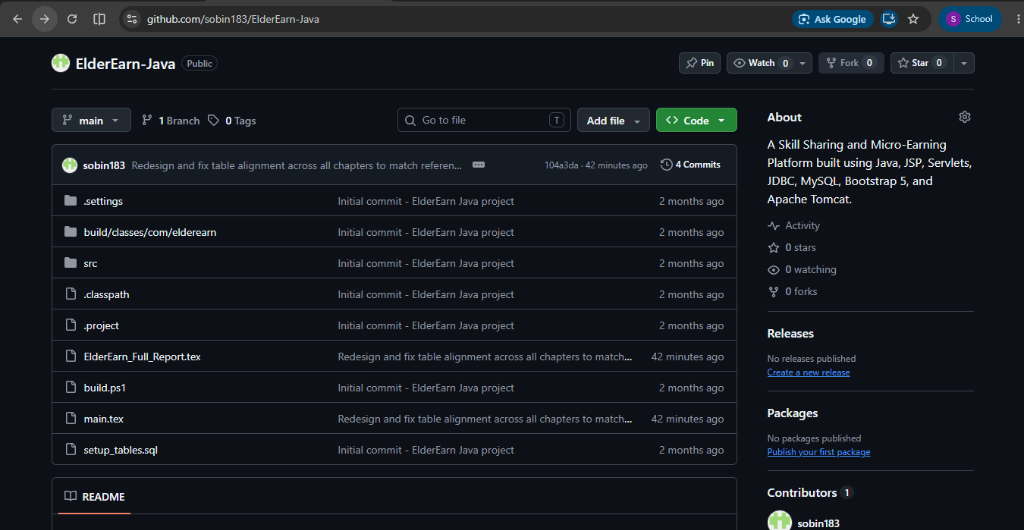
\includegraphics[width=0.88\textwidth]{gitlog.png}
\caption{GitHub Version Control Commit History and Repository Log}
\label{fig:screen_gitlog}
\end{figure}

The commit history documents continuous engineering progress, including database schema initialization, servlet controllers, security filters, and automated Selenium test integration.

\begin{table}[H]
\centering
\small
\caption{Summary of Key Git Repository Commits and Milestones}
\label{tab:git_commits}
\begin{tabularx}{\textwidth}{|L{2.0cm}|L{2.5cm}|L{3.2cm}|J|}
\hline
\textbf{Commit ID} & \textbf{Date} & \textbf{Author} & \textbf{Commit Message / Milestone} \\ \hline
\texttt{e4f1a2c} & 2026-08-14 & Sobin Thankachan & Initial project commit with directory structure \\ \hline
\texttt{8b3d91f} & 2026-08-20 & Sobin Thankachan & Added MySQL 8.0 schema and database connection utility \\ \hline
\texttt{c1a7e44} & 2026-08-28 & Sobin Thankachan & Implemented LoginServlet and role authentication \\ \hline
\texttt{5f2e809} & 2026-09-02 & Sobin Thankachan & Added course management and video upload handler \\ \hline
\texttt{9d4b671} & 2026-09-08 & Sobin Thankachan & Integrated escrow wallet and atomic transaction logic \\ \hline
\texttt{3a8f102} & 2026-09-12 & Sobin Thankachan & Automated Selenium test suites and UI accessibility \\ \hline
\end{tabularx}
\end{table}

\end{document}
